\begin{figure}
	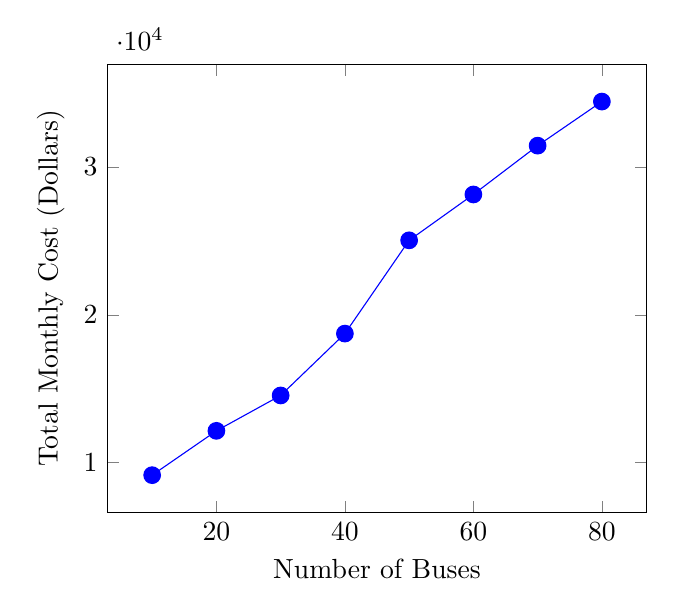
\begin{tikzpicture}
		\begin{axis}[xlabel=Number of Buses, ylabel=Total Monthly Cost (Dollars), legend pos=north west, legend style={nodes={scale=0.7}}]
			\addplot[blue] coordinates {
				(10,  9145.19)
				(20, 12145.78)
				(30, 14540.29)
				(40, 18728.08)
				(50, 25041.29)
				(60, 28145.93)
				(70, 31450.49)
				(80, 34434.68)}; 
			\addplot[blue, only marks, mark size=3pt] coordinates {
				(10,  9145.19)
				(20, 12145.78)
				(30, 14540.29)
				(40, 18728.08)
				(50, 25041.29)
				(60, 28145.93)
				(70, 31450.49)
				(80, 34434.68)}; 
			%\legend{Proposed, Baseline, He et al.}
		\end{axis}
	\end{tikzpicture}
	\caption{Monthly Cost without contention}
	\label{fig:scalabilityCost}
\end{figure}


